% Docker Meetup at MfN, 24 April 2018
% Running wikis at the Museum with Docker - past, present and future
% Alvaro Ortiz-Troncoso
% 
% Template:
% see https://en.wikibooks.org/wiki/LaTeX/Presentations

\documentclass[13pt]{beamer}
\usepackage[utf8]{inputenc}
\usepackage{graphicx}
\usepackage{xcolor}

\definecolor{mfn_green}{HTML}{A1BF23}
\setbeamercolor{title}{fg=black}
\setbeamerfont{title}{family=\sffamily,series=\bf}
\setbeamercolor{frametitle}{fg=black}
\setbeamerfont{subtitle}{family=\sffamily,shape=\itshape}
\beamertemplatenavigationsymbolsempty
\setbeamertemplate{footline}[page number]
\setbeamertemplate{itemize item}{\color{mfn_green}$\blacktriangleright$}
\setbeamertemplate{caption}{\tiny \insertcaption}
\setbeamersize{text margin left=5mm,text margin right=5mm}

% Running wikis at the Museum with Docker: past, present and future The Museum outputs exhibitions, science papers, conferences, and so much more. None of this would be possible without cooperation between researchers, designers, organizers and of course admins and developers. Wikis were introduced at the Museum in 2014 as an %experiment to improve  cooperation within project teams. I'll talk about how Docker solves many of the problems of running a bunch of wikis on a string, and also about pending questions we are currently trying to answer. I am a computer scientist and joined the Museum in 2014. I have worked at the Technische Universität Berlin and at Waag Technology & Society in Amsterdam.

\title
{Running wikis at the Museum with Docker}
\subtitle{past, present and future}
\author
{Alvaro Ortiz-Troncoso}
\date
{Docker Meetup at Museum für Naturkunde Berlin, 2018}
\subject{Computer Science}

\begin{document}

% 1. Titelseite
{
  \logo{
\includegraphics[height=1cm]{mfn_logo_klein.png}\vspace{220pt}}
  \frame{\titlepage}
}

% 2. Das Museum
% This talk is about our experience with combining Docker and wikis at the Museum. First I'll talk shortly about what we do at the Museum, and how we do it. The Museum is a very dynamic environment, and working here is probably very different from what most people imagine. Then I'll talk about running wikis with Docker. I'll go into the reasons for adopting Docker, both organisational and technical. Finally, I'll talk about plans for the future. Particularly regarding our plans, I'm very interested in hearing your feedback, criticism, and ideas.
% Dieser Vortrag handelt von unsere Erfahrung mit der Kombination von Docker und Wikis am Museum. Zuerst werde ich kurz sprechen über was wir am tun Museum, und über wie wir es tun. Das Museum ist ein sehr dynamisches Umfeld, und hier zu arbeiten ist vielleicht anders, als die meisten Personen sich vorstellen. Danach werde ich über Wikis und Docker sprechen. Ich werde die Gründe durchnehmen, wieso wir uns für Docker entschieden haben, sowohl organisatorisch als auch technisch. Schließlich werde ich sprechen über unsere Zukunftspläne. Besonders darüber freue ichh mich über Feedback, Anregungen, Kritik und Ideen. 
\begin{frame}
  \frametitle{Das Museum / \textcolor{mfn_green}{The Museum}}
  \begin{figure}
    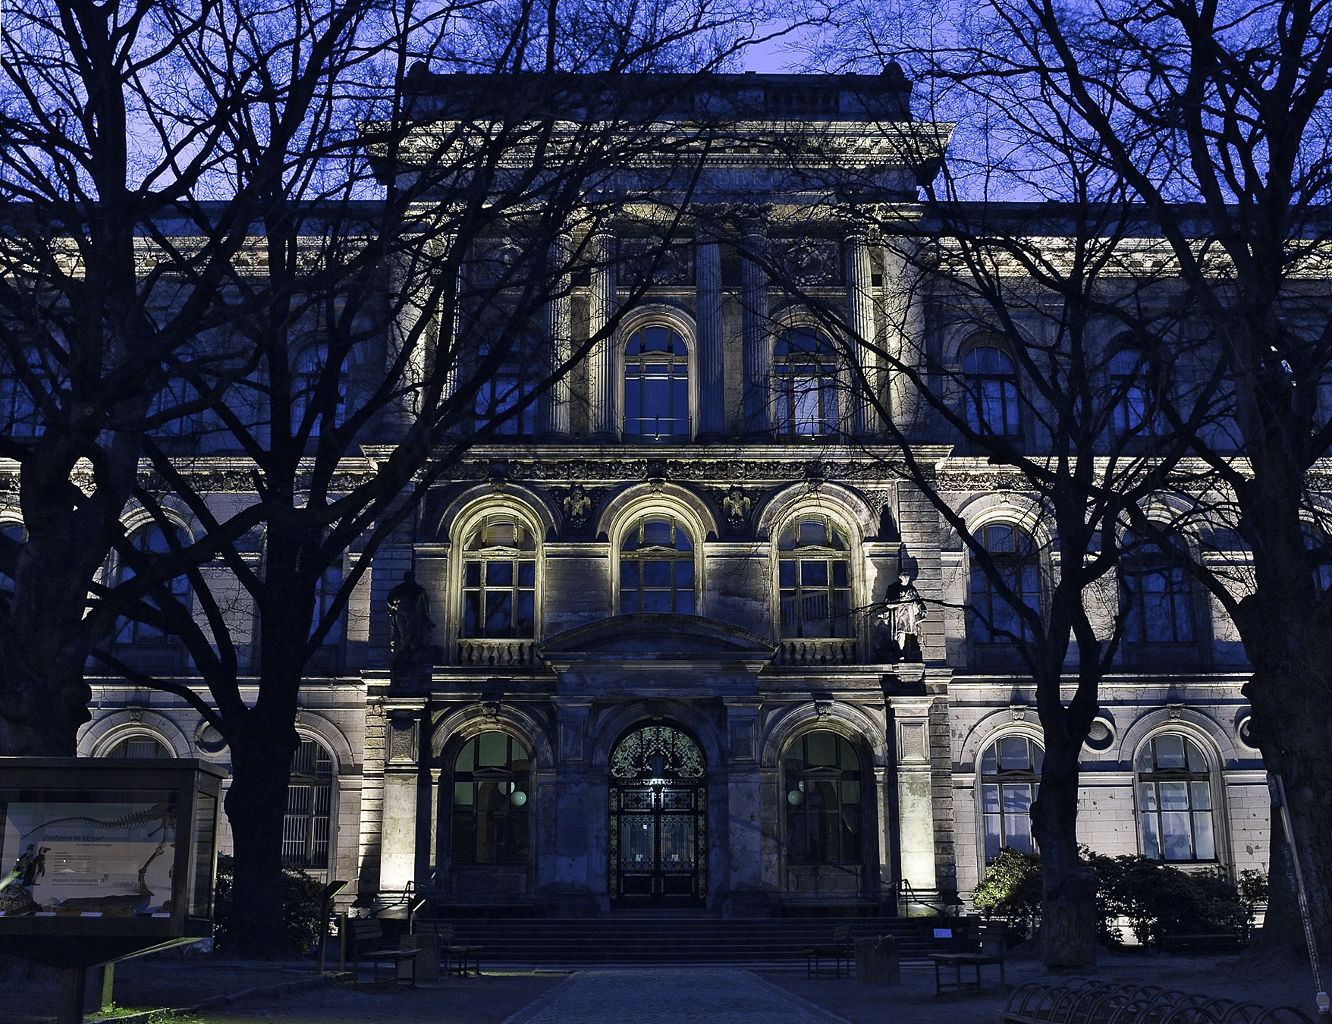
\includegraphics[height=70mm]{Gebaeude_Nacht.jpg}
    \caption{\textcopyright Antje Dittmann, Museum für Naturkunde Berlin, 2009. CC-by-sa}
  \end{figure}
\end{frame}

% 3. Ausstellung
% Most people think the Museum is the exhibition. This is partly true, but there is much more going on behind the scenes. Of course, many people know that museums cannot display everything they have. But most people are unaware of the amount of research that is carried out on the collection.
% Die meisten Personen denken, dass das Museum und die Ausstellung gleichzusetzen sind. Das entspricht nur zum Teil die Wahrheit. Die meisten Personen sind sich davon bewusst, das nicht alles, was das Museum besitzt, ausgestellt werden kann, aber die Menge an Forschung, die hinten den Kulissen betrieben wird, ist den meisten Personen nicht bewusst.
\begin{frame}
  \frametitle{Die Ausstellung / \textcolor{mfn_green}{The exhibition}}
  \begin{figure}
  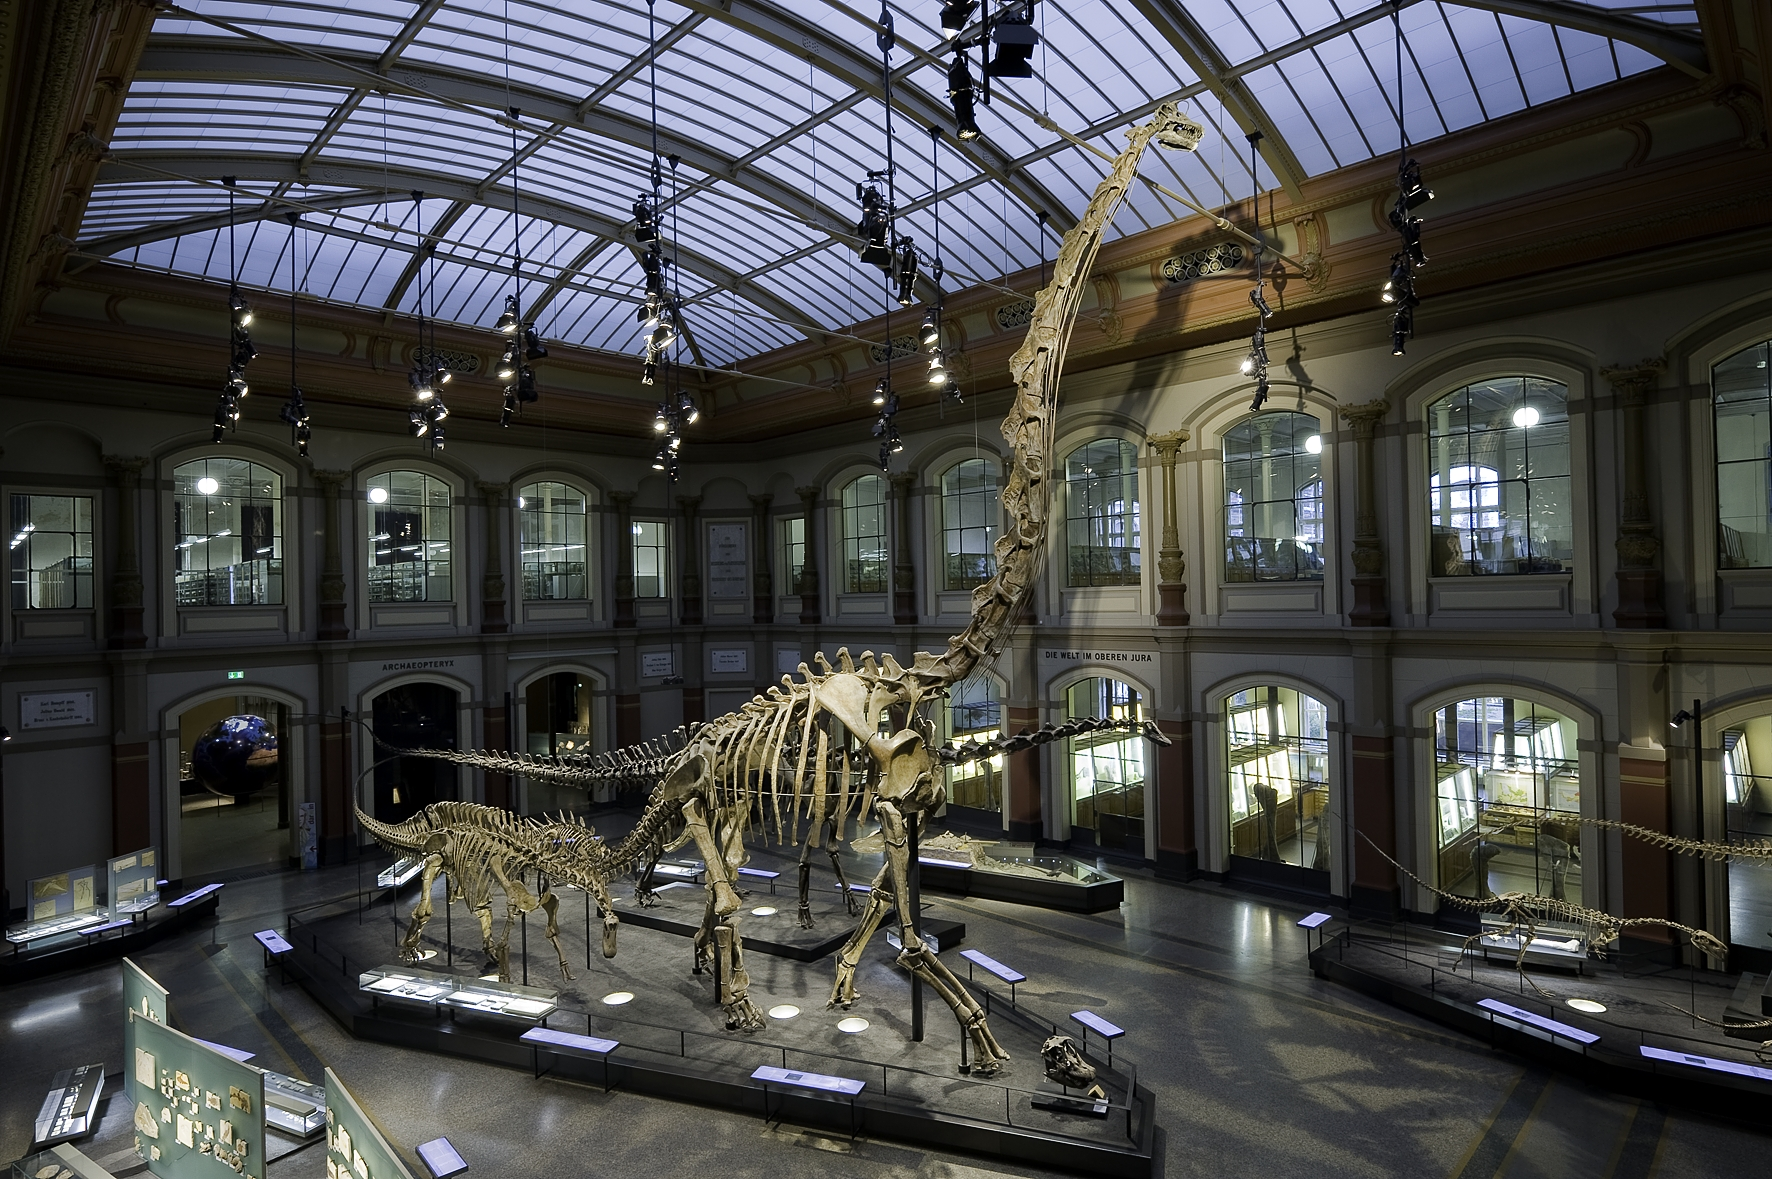
\includegraphics[height=70mm]{Brachiosaurus_02_15cm.jpg}
  \caption{\textcopyright Antje Dittmann, Museum für Naturkunde Berlin, 2009. CC-by-sa}
  \end{figure}
\end{frame}

% 4. Einige Zahlen
% Almost 500 persons work at the museum, including scientists, students, lab technicians, software developers and so on. As in any science institution, output can be measured by the number of publications. These include science publications but also books and articles in magazines. There are currently 51 research projects actively working on the collection.
% Fast 500 Personen arbeiten m Museum, das sind WissenschaftlerInnen, StudentInnen, Labor TechnikerInnen, EntwicklerInnen und so weiter. Wie in jedem Wissenschaftsinstitut kann die Produktion an der Menge der Publikationen gemessen werden. Mit Publikationen sind hier sowohl wissenschaftliche Artikel in spezialisierte Zeitschriften als Ausstellungskataloge und so weiter gemeint. Zur Zeit sind 51 Forschungsprojekte am Museum aktiv, und erforschen die Sammlung.
\begin{frame}
  \frametitle{ Einige Zahlen / \textcolor{mfn_green}{Some numbers}}

  \begin{itemize}
  \item{Personal: 289, Studenten: 209}
  \item{Publikationen: 222 / Jahr (2016)}
  \item{Aktuell erforschen 51 Projekte die Sammlung}
  \end{itemize}
  
  \begin{itemize}
  \item{\textcolor{mfn_green}{Staff: 289, Students: 209}}
  \item{\textcolor{mfn_green}{Publications 222 / year (2016)}}
  \item{\textcolor{mfn_green}{Currently 51 projects are researching the collection}}
  \end{itemize}
  \bigskip
  \begin{center}\tiny{Unsere Wissenschaft / Our Science, DOI: 10.7479/3dwq-8a7g}\end{center}
\end{frame}

% 5. Forschungsprojekte
% Here are some examples of research projects: the Museum hosts a number of laboratories, where research is carried out in many fields, such as genetics. The Museum is using 3D-scanners to digitise the collection. The Museum is also involved in ecological projects, for example in mapping the biological diversity in specially interesting region. Geologists at the Museum are modelling planetary impacts, and meteorites. The Museum also developed an App, that can be downloaded from the App-Store, that helps to identify birds by song and plants using a mobile phone. There are just a few almost randomly chosen examples of projects on our Website. % Hier sind einige Beispiele von Forschungsprojekte: im Museum sind mehrere Labore untergebracht, wo verschiedene Arten von Forschung betrieben wird, zum Beispiel zu Genetik. Das Museum benutzt 3D-Scanners um die Sammlung zu digitalisieren. Das Museum ist auch in ökologische Projekte involviert, zum Beispiel zur Biodiversitätsforschung in besonders interessante Gebiete. Geologen am Museum erforschen die Folgen von Meteoriteneinschläge und benutzen dazu Computersimulationen. Dsa Museum hat ein App entwickelt, das im App-Store heruntergeladen werden kann, das bei der Bestimmung von Pflanzen und Vogestimmen helfen kann. Diese sind fast zufällig ausgewählte Projekte auf unsere Webseite.
\begin{frame}
  \frametitle{Forschungsprojekte / \textcolor{mfn_green}{Research projects}}
  \begin{figure}
  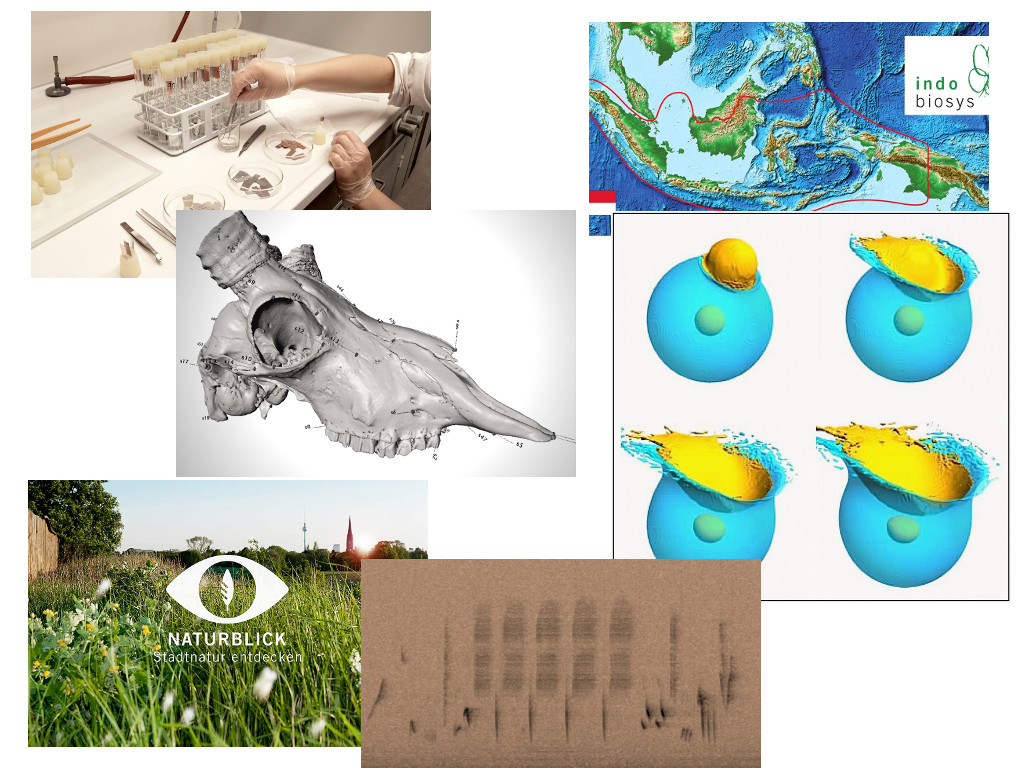
\includegraphics[height=70mm]{Forschung.jpg}
  \caption{https://www.museumfuernaturkunde.berlin/}
  \end{figure}
\end{frame}

% 6. Was macht ein Projekt aus?
% On the one hand, the Museum is meant to preserve and curate the collection, forever. On the other hand, we do all this exiting, dynamic stuff. This is possible because research projects are set up in a very similar way to projects in a start-up. A project basically needs 3 things: funding, a time plan (a project has a beginning and an end), and most importantly a team. Research teams at the Museum often include a researcher and collaborators from many different fields, such a software developers, system administrators, management people, designers or photographers, lab technicians and so on.
% Einerseits soll das Museum die Sammlung konservieren und kuratieren, für die Ewigkeit. Andererseits, passieren hier all diese aufregende, dynamische Dinge. Das ist möglich, weil wir in Projekte arbeiten, die im Wesen mit Projekte in einer Start-up nicht zu unterscheiden sind. Ein Projekt brauch im Grunde genommen nur 3 Dinge: Finanzierung, Zeitplan (Projekte haben einen Anfang und ein Ende) und Team. Forschungsteams am Museum bestehen typischerweise aus Wissenschaftler und Mitarbeiter aus verschiedenen Disziplinen, wie zum Beispiel Software-EntwicklerInnen, System-Administratoren, Projektmanagers, Designer, Fotografen, LabortechnikerInnen usw.
{
\setbeamercolor{background canvas}{bg=mfn_green}
\setbeamercolor{frametitle}{fg=black}
\begin{frame}
  \frametitle{Was macht ein Projekt aus? \\ \textcolor{white}{What does it take to launch a project?}}
  \begin{figure}
  \includegraphics[height=70mm,trim=4 4 4 4,clip]{Projekt.png}
  \end{figure}
  \bigskip
\end{frame}
}

% 7. Kooperation
% Cooperation is necessary for at least 3 reasons: a team that is made of persons coming from different fields and specialities, needs to come to a common understanding of what it is they wish to achieve. For example, "success" for a scientist might be something totally different than "success" for a manager. Cooperation is also necessary to deliver on time. As anybody who has worked on a project can tell, there is never enough time. Cooperation is also necessary to work efficiently and deliver within budget.
% Kooperation ist nötig aus mindestens drei Gründe: ein Team, das aus Mitarbeitern mit verschiedenen Hintergründe und Spezialisierungen besteht, muss zu einem gemeinsamen Verständnis kommen, was die Ziele des Projekts sind. Zum Beispiel kann "Erfolg" für einem Wissenschaftler was völlig anderes sein als "Erfolg" für einen Manager. Kooperation ist auch nötig, um das Zeitplan einzuhalten. Jeder, der an einem Projekt gearbeitet hat, weißt, das die Zeit nie reicht. Kooperation ist aber auch nötig, um innerhalb des Kostenrahmens zu bleiben, denn wer kooperiert arbeitet auch effizienter.
\begin{frame}
  \frametitle{Kooperation / \textcolor{mfn_green}{Cooperation}}

  \begin{itemize}
  \item{Gemeinsames Verständnis der Projektziele}
  \item{Innerhalb des Zeitrahmens zum Ergebnis kommen}
  \item{Den Kostenrahmen nicht überschreiten - Effizient arbeiten}
  \end{itemize}
  
  \begin{itemize}
  \item{\textcolor{mfn_green}{Common understanding of project goals}}
  \item{\textcolor{mfn_green}{Deliver on time}}
  \item{\textcolor{mfn_green}{Be efficient to finish within budget}}
  \end{itemize}
\end{frame}

%%%%%%%%%%%%%%%
%
% The past
%
%%%%%%%%%%%%%%%

% 8. In der Vergangenheit
\begin{frame}
  \frametitle{In der Vergangenheit / \textcolor{mfn_green}{In the past}}
  \begin{figure}
    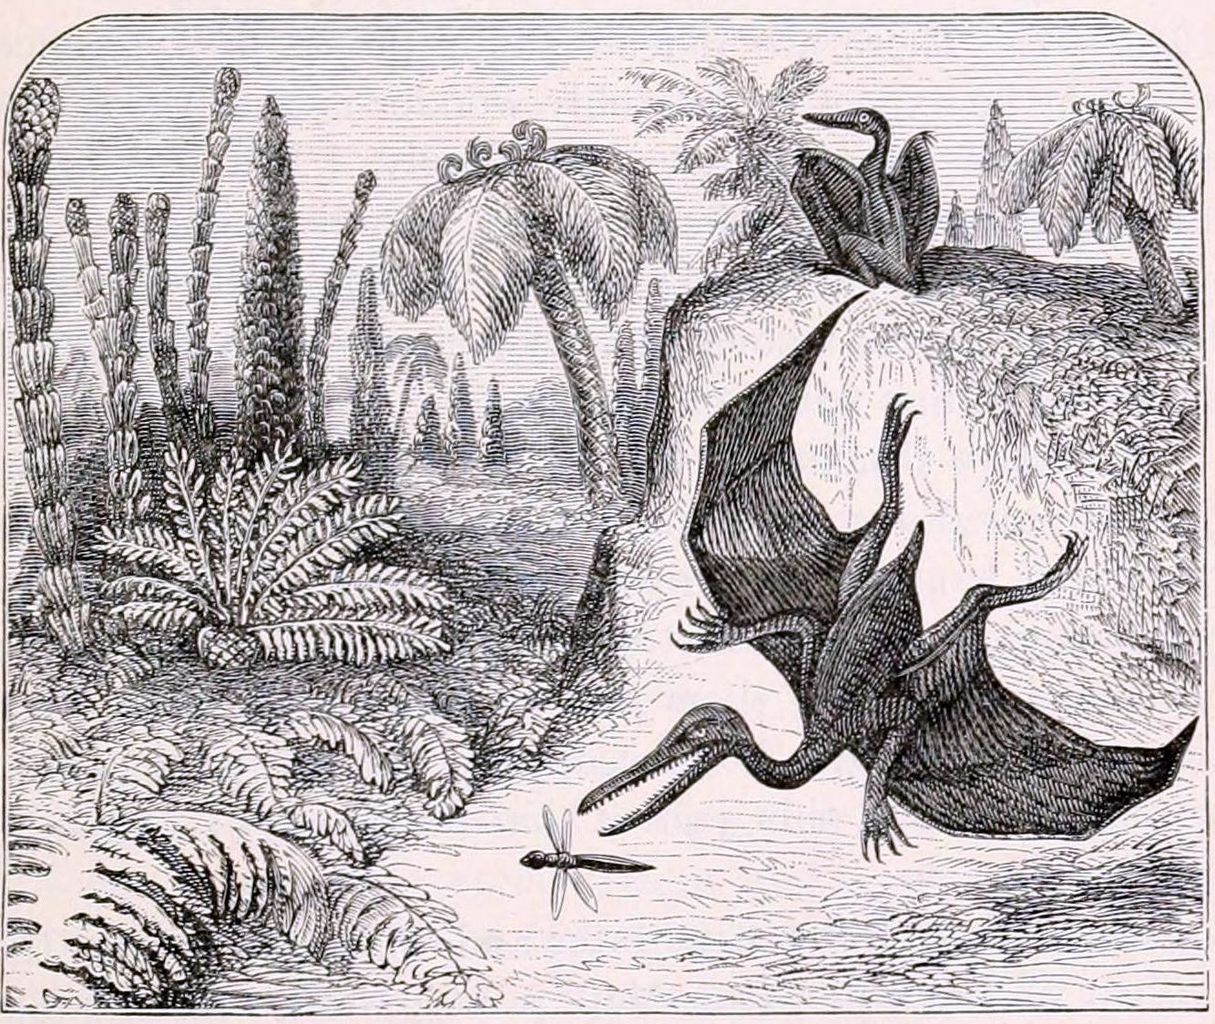
\includegraphics[height=70mm]{Ideal_Landscape_of_a_Prehistoric_Age.jpg}
    \caption{Quackenbos, J.D., 1886. \textit{Illustrated School History of the World}. D. Appleton.}
  \end{figure}
\end{frame}

% 9. Word .doc Hölle
% In the past, the only way to cooperate was through exchanging paper documents. Unfortunately, many people still think this way, except that Word documents have replaced paper. So a primitive way of cooperating is to place a Word document on a shared drive and to email the documents address to your collaborators. As Word does not support collaboration, this means that a document that is opened for editing by one person cannot be edited by anyone else. As this happens very often, people have taken to sending documents as email attachments, which is a definitive receipt for final chaos.
% Früher war Kooperation durch hin-und-her schicken von Papierunterlagen geprägt. Leider, gibt es immer viele Personen, die diese Art und Weise eins-zu-eins in die digitale Welt übernommen haben. Eine primitive Art der Kooperation ist, Word Dokumente auf eine gemeinsam benutzte Festplatte zu speichern, und die Adresse des Dokuments an den Projektmitarbeitern per Email zu verschicken. Weil Word keine Kooperationsfunktionen hat, bedeutet es, dass ein Dokument, das von einem Mitarbeiter geöffnet ist, von den anderen nicht bearbeitet werden kann. Weil das sehr oft passiert, ist es Usus geworden, Word Dokumente als Beilage zu Emails zu verschicken, ein Rezept für endgültiges Chaos.
{
\setbeamercolor{background canvas}{bg=mfn_green}
\setbeamercolor{frametitle}{fg=black}
\begin{frame}
  \frametitle{Word\textsuperscript{\tiny\textregistered} .doc Hölle /
    \textcolor{white}{Word\textsuperscript{\tiny\textregistered} .doc hell}}
  \begin{figure}
  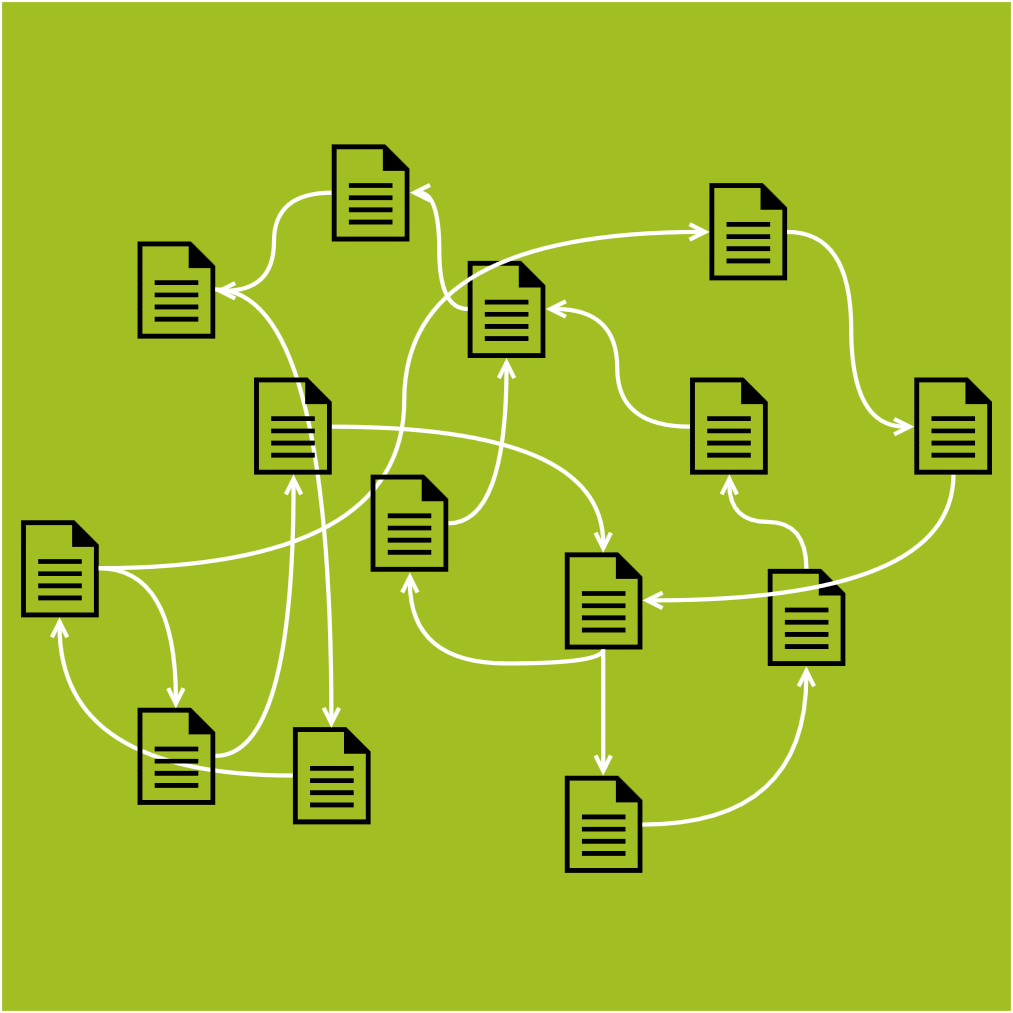
\includegraphics[height=70mm,trim=4 4 4 4,clip]{Docs.png}
  \end{figure}
\end{frame}
}

% 10. Nichts gegen Word aber...
% Although Word is quite a good programme, when it comes to cooperation it has some very clear disadvantages: There is no way to know which one of the document copies is the final version, or if there are several versions, there is no way to automatically merge documents. Word does not provide a transparent mechanism to follow who wrote which part of a document. Authorship is very important for researchers, as researchers build up their scientific reputation by publishing. Another important drawback of Word is that it is a proprietary format. The Museum has been around since 1889 and will survive not only all of us, but very probably also Microsoft, and what happens then?
% Obwohl Word ein ziemlich gutes Programm ist, hat es für kooperatives Arbeiten gewisse Nachteile: es gibt keine Möglichkeit herauszufinden, welche der Kopien des Dokuments, die per Email in Umlauf gebracht sind, die endgültige Fassung ist. Oder, wenn es mehrere Fassungen des Dokuments gibt, gibt es aber keine Möglichkeit, die verschiedenen Fassungen zusammenzufügen. Word bietet keine Möglichkeit zur Verfolgung der Autorschaft des Dokuments oder Teile davon. Autorschaft ist essentiell für ForscherInnen, denn ihre wissenschaftliche Reputation basiert darauf. Ein andere Nachteil von Word ist, dass es sich um proprietäre Software handelt. Dsa Museum existiert seit 1889, und wird nicht nur uns überleben, sondern mit aller Wahrscheinlichkeit auch Microsoft, und was ist dann?
\begin{frame}
  \frametitle{Nichts gegen Word\textsuperscript{\tiny\textregistered} aber... \\
    \textcolor{mfn_green}{Absolutely nothing against Word\textsuperscript{\tiny\textregistered}, however, ...}}
  \begin{itemize}
  \item{Keine Versionierung: wer hat die Endfassung?}
  \item{Kein Dokumentverlauf: wer hat was geschrieben?}
  \item{Proprietäre Software: Anbieterabhängigkeit}
  \end{itemize}
  
  \begin{itemize}
  \item{\textcolor{mfn_green}{No versioning: who has the final version}}
  \item{\textcolor{mfn_green}{No document history: who wrote what?}}
  \item{\textcolor{mfn_green}{Proprietary software: vendor lock-in}}
  \end{itemize}
\end{frame}

%%%%%%%%%%%%%%
%
% The present
%
%%%%%%%%%%%%%%

% 11 Beispiel Panda-Wiki
% For these reasons, the Museum decided to set up a cooperation environment. When I joined the Museum in 2014, my first job was to experiment with wikis to create such an environment. There are currently 24 wikis at the Museum, here is an example: the wiki of the Panda exhibition. This wiki is interesting because it went through the life-cycle of a whole project: during project planing, it was used to write texts for the labels in the exhibition, and to gather material for the exhibition catalogue. During the exhibition (2015), it was made public and was used as exhibition website. After the exhibition, the wiki can now be used as exhibition archive.
% Aus diesen Gründen hat das Museum entschieden, eine Kooperationsumgebung aufzusetzen. Als ich am Museum in 2014 angefangen habe, war mein erster Auftrag mit Wikis zu experimentieren, um eine Kooperationsumgebung zu schaffen. Heutzutage gibt es 24 Wikis am Museum. Hier ist ein Beispiel: das Wiki der Panda Ausstellung. Dieses Wiki ist interessant weil es alle Stadien eines Projetkzyklus durchlaufen hat. Während der Planung der Ausstellung wurde das Wiki benutzt, um die Texte der Ausstellung zu schreiben, und um Materialien zu sammeln für das Ausstellungskatalog. Während der Ausstellung (2015), wurde das Wiki veröffentlicht und diente als Ausstellungswebseite. Nach der Ausstellung dient das Wiki als Ausstellungsarchiv.
\begin{frame}
  \frametitle{Konkretes Beispiel: das Panda-Wiki\\\textcolor{mfn_green}{A specific example: the Panda wiki}}
  \begin{figure}
    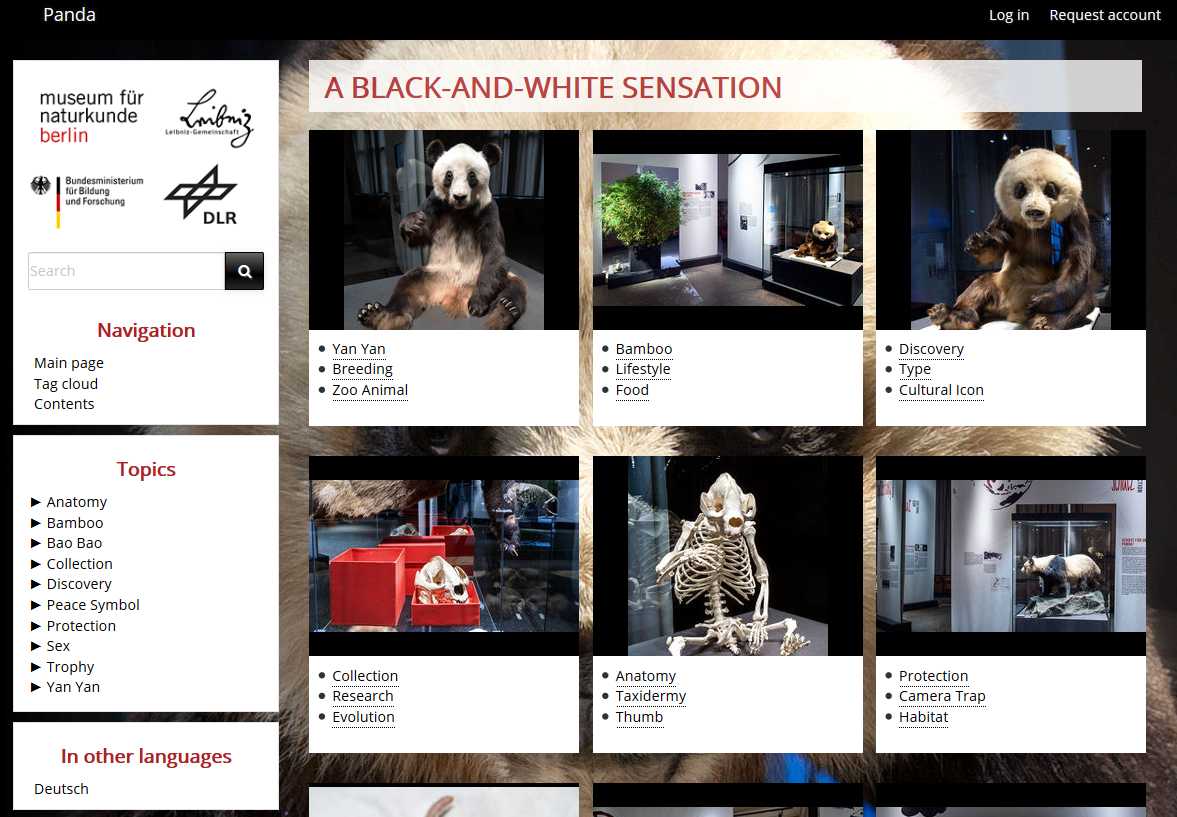
\includegraphics[height=60mm]{panda.png}
    \caption{http://biowikifarm.net/v-mfn/panda}
  \end{figure}
\end{frame}

% 12. Wikis am Museum
% Research projects at the Museum may use a wiki to support collaboration within a team, if they wish to do so. Although projects at the Museum can be of very different kinds, the wikis have some requirements in common. Two important requirements are: wikis are by default private. Scientists are sometimes reluctant to share their data and results before their research has been published, as scientists are specially rewarded for publishing unheard-off results. These are the rules of the game in academia nowadays. The second important requirement is that wikis should be semantic. This means that our wikis are capable of storing free-form texts, in a similar way than Wikipedia can deal with texts, but can also store structured data. Information in the wiki can then be queried in various ways, and that increases value of the information stored in the wiki.
% Forschungsprojekte am Museum können ein Wiki benutzen, wenn sie das wünschen. Obwohl Projekte im Museum sehr verschieden sein können, haben die Wikis dennoch gemeinsame Anforderungen. Die Zwei wichtigste Anforderungen sind: die Wikis sind standardmäßig privat. WissenschaftlerInnen sind manchmal abgeneigt, Forschungsergebnisse zu teilen, bevor diese in einer wissenschaftlichen Zeitschrift publiziert worden sind, weil WissenschaftlerInnen besonders honoriert werden, wenn sie völlig neue Ergebnisse publizieren. Das sind die Regeln des Wissenschaftsbetrieb heutzutage. Die zweite wichtige Anfordeung ist, dass die Wikis semantisch sein sollen. Das heißt, dass unsere Wikis nicht nur mit Freiformtexte umgehen können, sondern auch mit strukturierten Daten. Informationen im Wiki kann auf verschiedene Art und Weisen durchsucht werden, was ihre Nützlichkeit steigert.
\begin{frame}
  \frametitle{Wikis am Museum / \textcolor{mfn_green}{Wikis at the Museum}}

  \begin{itemize}
  \item{Forschungsprojekte können ein Wiki nutzen, sofern sie es wünschen}
  \item{Wikis sind standardmäßig privat, können aber zum Teil oder im Ganzen geöffnet werden}
  \item{Wikis sind semantisch: sie können sowohl mit Freiformtexten als auch mit strukturierten Daten umgehen}
  \end{itemize}
  
  \begin{itemize}
  \item{\textcolor{mfn_green}{Research projects may use a wiki if they wish to do so}}
  \item{\textcolor{mfn_green}{Wikis are private by default, but may be made public in part or in whole}}
  \item{\textcolor{mfn_green}{Wikis are semantic, so can be used with plain texts as well as with structured data}}
  \end{itemize}
\end{frame}

% 13. Die derzeitige Praxis
% In a nutshell, running projects requires cooperation. Cooperation has to be supported by a cooperation environment. Setting up a collaboration environment requires software infrastructure and processes. I'll go into more detail on the steps of this process on the next slide, and also into the problems this process has. Doing things this way has a very important advantage: a clear separation of concerns and responsibilities between the system administrators and the developers. System administrators are Museum staff, and they can concentrate on building the Museum's infrastructure, which is what they do best. Developers are temporary project staff or external contractors, and the can concentrate on pushing their project forward.
% Zusammengefasst, um Projekte zu betreiben ist Kooperation gefragt. Kooperatin muss von einer Kooperationsumgebung unterstützt werden. Um eine Kooperationsumgebung aufzusetzen werden eine Infrastruktur und Prozesse benötigt. Ich werde die Details des Prozess in der nächsten Slide zeigen, und auch auf die Probleme eingehen, die dieses Prozess mit sich bringt. Diese Art von Arbeit hat dennoch ein großes Vorteil: ene deutliche Trennung von den Belangen und Verantwortlichkeiten zwischen EntwicklerInnen und Admins. Admins sind Museumsangestellte, und sie können sich auf das Ausbauen einer Infrastruktur konzentrieren. EntwicklerInnen sind temporäre Projektangestellte, manchmal sogar externe Mitarbeiter, und sie können sich darauf konzentrieren, ihr Projekt voranzutreiben.
\begin{frame}
  \frametitle{Die derzeitige Praxis / \textcolor{mfn_green}{The current practice}}
  \begin{figure}
    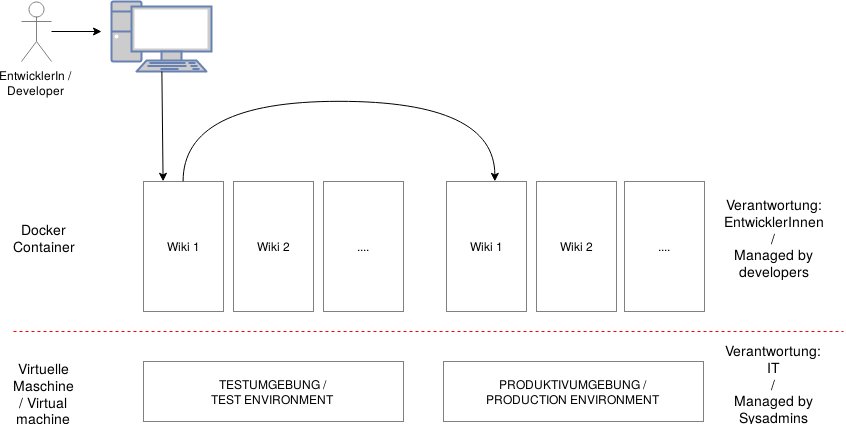
\includegraphics[width=110mm]{docker_wikis.png}
  \end{figure}
\end{frame}

% 14. Rolloutprozess
% A detailed look at the roll-out process, as it is implemented now. The current practice at the Museum is that new wikis are first build as a Docker image by a developer, at the developers desktop computer. Then the Docker images are uploaded to a test server for testing. If they pass the tests, the images are deployed to the production server.
% dsa Rollout-Prozess im Detail, so wie es zur Zeit noch implementiert ist. Die derzeitige Praxis am Museum ist, dass Wikis zuerst als Docker Image gebaut werden auf dem Desktop Rechner der EntwicklerInnen. Die Docker Images werden dann auf dem Testserver hochgeladen und getestet. Wenn die Tests bestanden sind, werden die Images auf den Produktivserver eingesetzt.
\begin{frame}
  \frametitle{Rolloutprozess / \textcolor{mfn_green}{Roll-out process}}

  \begin{figure}
    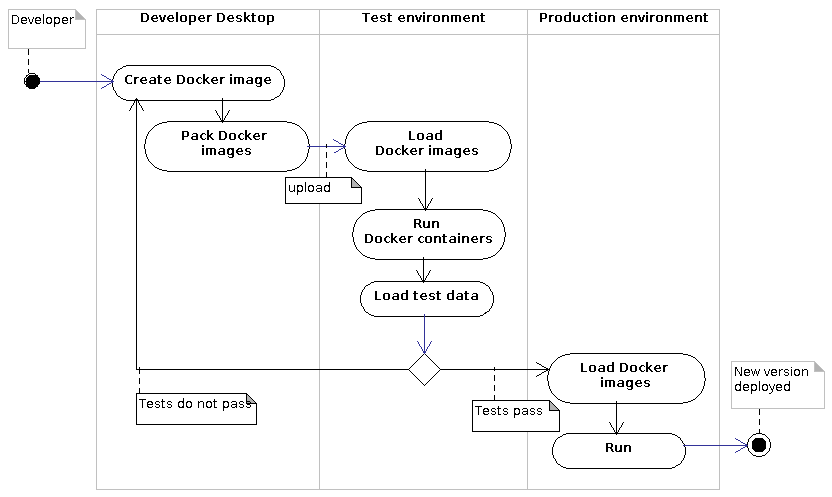
\includegraphics[width=\textwidth]{deploy_wiki_uml.png}
  \end{figure}

\end{frame}

%%%%%%%%%%%%%%
%
% The future
%
%%%%%%%%%%%%%%

% 15. Blick in die Zukunft
\begin{frame}
  \frametitle{Blick in die Zukunft \\ \textcolor{mfn_green}{The shape of things to come}}
  \begin{figure}
    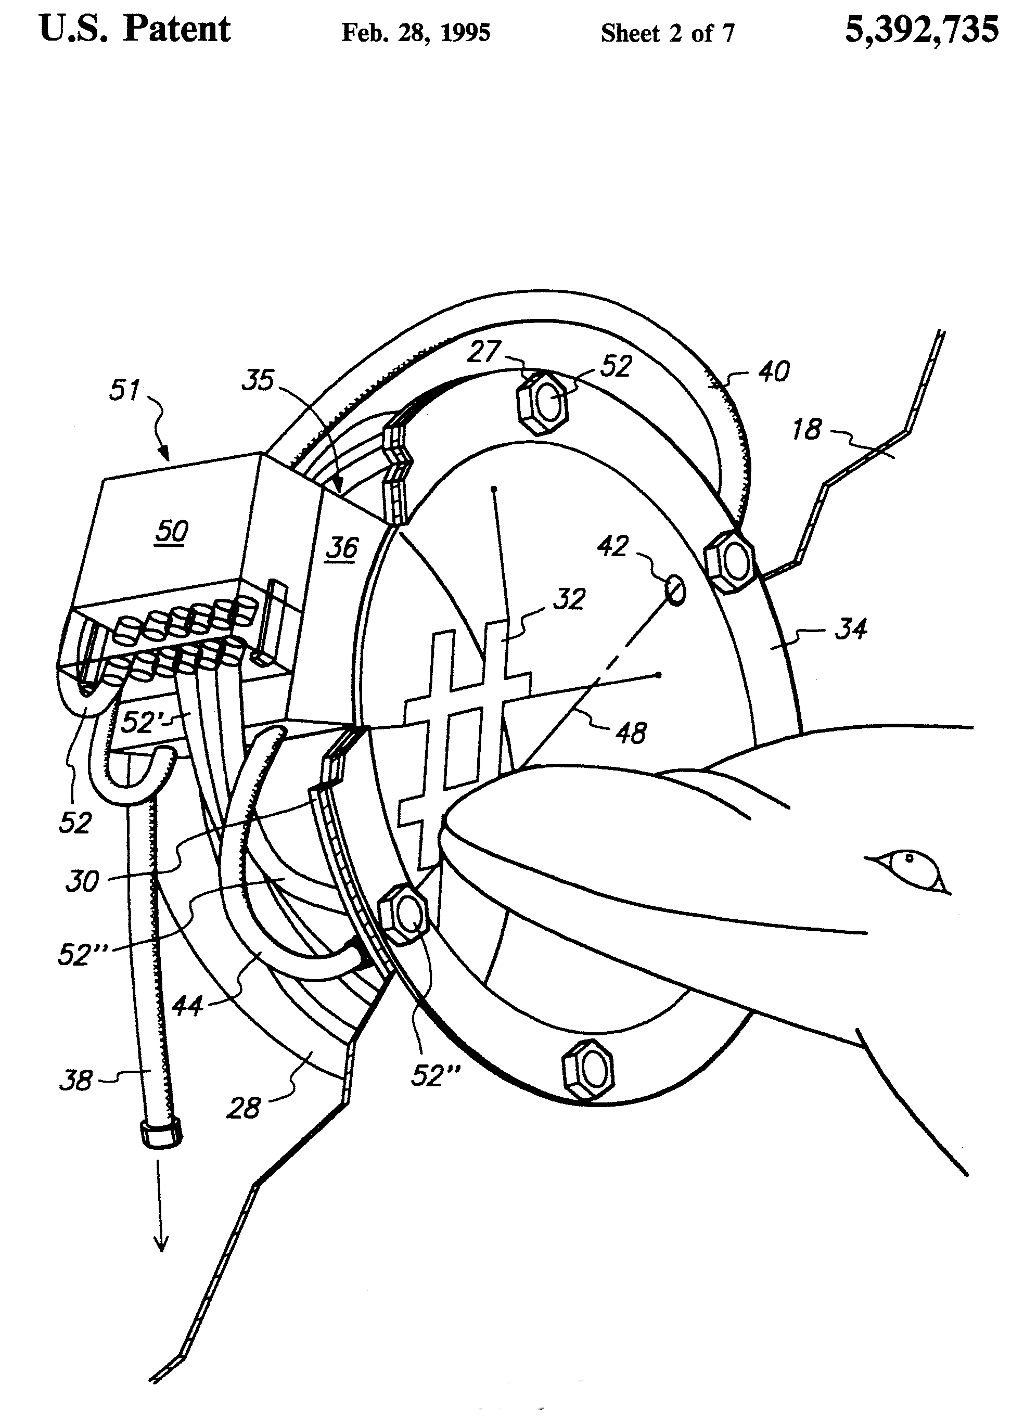
\includegraphics[height=60mm]{marine_mammal_communication.png}
    \caption{Xitco Jr, M.J. et al, 1995. \textit{Marine mammal communication device}. U.S. Patent 5,392,735.}
  \end{figure}
\end{frame}

% 16. Problemzone
% As I'm sure some of you have noticed, the current roll-out process has some disadvantages. One is that the test environment is very prone to failure. As all developers use it, it is often broken and unavailable. Another problem is that much of this stuff is done either by hand or through self-written scripts. This takes time and is not easy to maintain.
% Der derzeitige Rollout-Prozess hat offensichtliche Nachteile. Einer davon ist, dass die Testumgebung seht störungsanfällig ist. Da alle Entwickler denselben Server nutzen, ist dieser oft kaputt oder nicht erreichbar. Ein anderes Problem ist, dass viel noch per Hand oder mithilfe von selbsgeschriebenen Skripten gemacht werden muss. Das kostet Zeit und ist nicht einfach zu Warten.
\begin{frame}
  \frametitle{Problemzone / \textcolor{mfn_green}{Problem zone}}
  \begin{figure}
    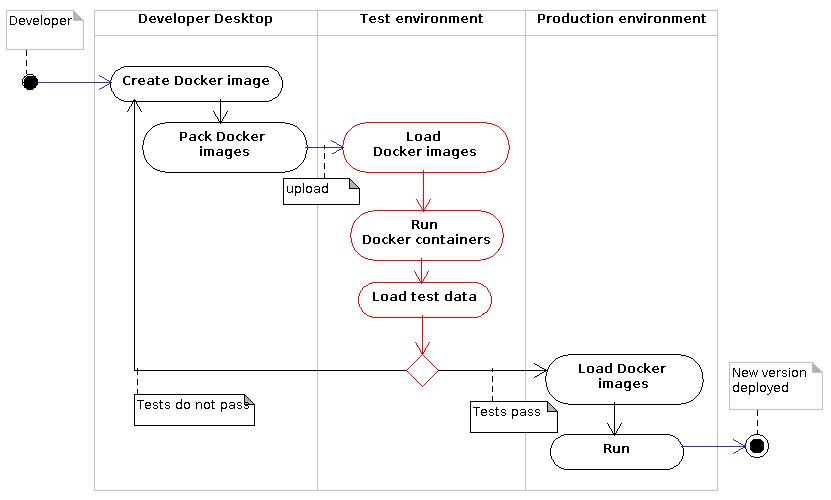
\includegraphics[width=\textwidth]{docker_wikis_problem_uml.png}
  \end{figure}
\end{frame}

% 17. Lösungsansatz
% My current priority is to streamline the roll-out process, by getting rid of the test environment and replacing it with continuous integration. Setting up continuous integration can be a lot of effort, but as anyone who has worked with continuous integration can tell, it is effort well spent. Continuous integration automates the roll-out process, renders testing more transparent, and once it is set up, it is just a mater of submit-and-forget. I am currently planing to use Jenkins to build the continuous integration pipeline. The first step in the pipeline would be to create a disposable virtual machine for testing, using Vagrant. Then the Docker containers would be deployed in the virtual machine, along with some test data. The tests can then run in Selenium. If the tests pass, the new images would be deployed to the production environment.
% Meine Priorität ist, um das Rollout zu optimieren. Ich will die Testumgebung durch Continuous Integration ersetzen. Continuous Integration aufzusetzen kann viel Arbeit bedeuten, aber jeder, der damit gearbeitet hat kann bezeugen, dass es sich am Ende lohnt. Continuous Integration automatisiert der Rollout-Prozess, macht testen transparent und wenn es einmal steht, ist sehr einfach zu bedienen. Mein jetziger Plan ist es, um Jenkins zu benutzen, um die Continuous Integration Pipeline steuern. Der erste Schritt des Pipeline wäre, um eine Einmahl-Virtuelle-Maschine zu schaffen, mithilfe von Vagrant. darauf werden die Docker Container zum testen auf der Virtuellen Maschine eingesetzt. Die Tests können in Selenium gesteuert weden. Wenn die Tests erfolgreich sind, können die nuen Images in der Produktivumgebung automatisch eingesetzt werden.
\begin{frame}
  \frametitle{Lösungsansatz / \textcolor{mfn_green}{Planed solution}}
  \begin{figure}
    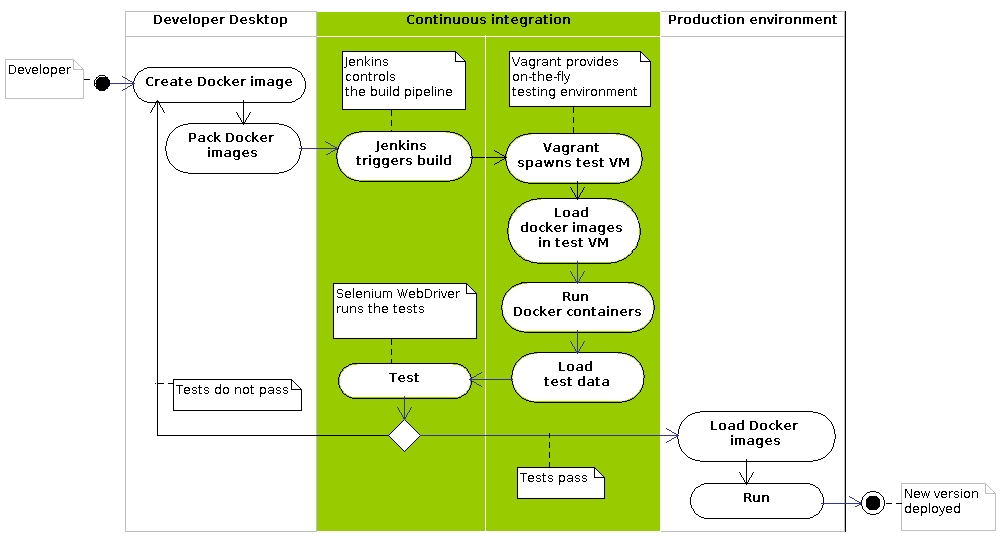
\includegraphics[width=\textwidth]{docker_wikis_integration.png}
  \end{figure}
\end{frame}

% 18. Kontaktdaten
\begin{frame}
  \frametitle{Kontaktdaten / \textcolor{mfn_green}{Contact information}}
  \begin{center}
    Alvaro Ortiz-Troncoso \\
    \medskip
    Email: Alvaro.OrtizTroncoso@mfn.berlin \\    
    \medskip
    Web: https://github.com/MfN-Berlin
  \end{center}
\end{frame}

\end{document}


